% mnras_template.tex 
%
% LaTeX template for creating an MNRAS paper
%
% v3.0 released 14 May 2015
% (version numbers match those of mnras.cls)
%
% Copyright (C) Royal Astronomical Society 2015
% Authors:
% Keith T. Smith (Royal Astronomical Society)

% Change log
%
% v3.0 May 2015
%    Renamed to match the new package name
%    Version number matches mnras.cls
%    A few minor tweaksto wording
% v1.0 September 2013
%    Beta testing only - never publicly released
%    First version: a simple (ish) template for creating an MNRAS paper

%%%%%%%%%%%%%%%%%%%%%%%%%%%%%%%%%%%%%%%%%%%%%%%%%%
% Basic setup. Most papers should leave these options alone.
\documentclass[fleqn,usenatbib]{mnras}

% MNRAS is set in Times font. If you don't have this installed (most LaTeX
% installations will e fine) or prefer the old Computer Modern fonts, comment
% out the following line
\usepackage{newtxtext,newtxmath}
% Depending on your LaTeX fonts installation, you might get better results with one of these:
%\usepackage{mathptmx}
%\usepackage{txfonts}

% Use vector fonts, so it zooms properly in on-screen viewing software
% Don't change these lines unless you know what you are doing
\usepackage[T1]{fontenc}
\usepackage{ae,aecompl}


%%%%% AUTHORS - PLACE YOUR OWN PACKAGES HERE %%%%%

% Only include extra packages if you really need them. Common packages are:
\usepackage{graphicx}	% Including figure files
\usepackage{amsmath}	% Advanced maths commands
\usepackage{amssymb}	% Extra maths symbols


%%%%%%%%%%%%%%%%%%%%%%%%%%%%%%%%%%%%%%%%%%%%%%%%%%

%%%%% AUTHORS - PLACE YOUR OWN COMMANDS HERE %%%%%

% Please keep new commands to a minimum, and use \newcommand not \def to avoid
% overwriting existing commands. Example:
%\newcommand{\pcm}{\,cm$^{-2}$}	% per cm-squared

\newcommand\halpha{H${\alpha}$}
\newcommand\n{[\ion{N}{II}]$\lambda$6584}
\newcommand\oi{[\ion{O}{III}]$\lambda$5007}
\newcommand\s{[\ion{S}{II}]$\lambda$6737}
\newcommand\si{$\sigma$}
\newcommand\kms{$^{-1}$}


%%%%%%%%%%%%%%%%%%%%%%%%%%%%%%%%%%%%%%%%%%%%%%%%%%

%%%%%%%%%%%%%%%%%%% TITLE PAGE %%%%%%%%%%%%%%%%%%%

% Title of the paper, and the short title which is used in the headers.
% Keep the title short and informative.
\title[Turbulence in GHRs]{Turbulence in giant HII regions}

% The list of authors, and the short list which is used in the headers.
% If you need two or more lines of authors, add an extra line using \newauthor
\author[J. García-Vázquez et al.]{
J. García Vázquez,$^{1}$\thanks{E-mail: jgarciav1600@alumno.ipn.mx}
J. Zsargo,$^{1}$
W. J. Henney$^{2}$
and H. O. Castañeda$^{1}$
\\
% List of institutions
$^{1}$Escuela Superior de Física y Matemáticas, Instituto Politécnico Nacional, Ciudad de México, México.\\
$^{2}$Instituto de Radioastronomía y Astrofísica, Universidad Nacional Autonoma de México, Apartado postal 3-72, 58090 Morelia, Michoacán, Mexico\\
}

% These dates will be filled out by the publisher
\date{Accepted XXX. Received YYY; in original form ZZZ}

% Enter the current year, for the copyright statements etc.
\pubyear{2021}

% Don't change these lines
\begin{document}
\label{firstpage}
\pagerange{\pageref{firstpage}--\pageref{lastpage}}
\maketitle

% Abstract of the paper
\begin{abstract}

We used the radial velocity field in H$\alpha$ emission with the aim of characterizing the turbulent state of the ionized gas in giant HII regions. For this purpose we use long-slit spectroscopy and Fabry-Perot observations obtained with the William Herschel Telescope. Each velocity sample was investigated applying the second order structure function. The correlations in our results are evidence that the velocity field can be consider in a turbulent state. This turbulent motions are described by a power-law with a mean index of 1.7 and a correlation length of 11 pc. The physical interpretation of the power-law behavior consider that an energy cascade is taking place in the photoionized gas.
\end{abstract}

% Select between one and six entries from the list of approved keywords.
% Don't make up new ones.
\begin{keywords}
HII regions -- ISM
\end{keywords}

%%%%%%%%%%%%%%%%%%%%%%%%%%%%%%%%%%%%%%%%%%%%%%%%%%

%%%%%%%%%%%%%%%%% BODY OF PAPER %%%%%%%%%%%%%%%%%%

\section{Introduction}

Different phases of the interstellar medium exhibits a chaotic behavior \citep{franco1999interstellar,elmegreen2004interstellar,scalo2004interstellar}. Velocity fields shows complex motions in the plane-of-sky (POS), and a non-thermal broadening on their spectral lines suggests disorder motions along the line-of-sight (LOS). The large lengths of astrophysical objects, ranging in scales from 10$^{6}$ to 10$^{17}$ m \citep{chepurnov2010extending}, and the high Reynolds numbers (Re), in the order of 10$^{4}$ and 10$^{9}$, of these objects \citep{lagrois2011} are related to the existence of turbulent flows. Despite numerous attempts in characterizing the turbulence in the photoionized gas, little is understood on the nature of the problem.   

The mathematical techniques developed by \citet{kolm1,heisenberg1951stability} were first applied to astronomical observations by \citet{von1951methode} and \citet{munch1958internal}. Their aim was to investigate the projection of a three-dimensional function into the plane of the sky. This procedure using the structure function allowed to determine a distinction between homogeneous turbulence and pure random velocity fluctuations, for the galactic HII region, the Orion Nebula. The analysis on the turbulence of the Orion Nebula was continued by \citet{castaneda1988} and \citet{1992ApJ...387..229O}. In more recent years \cite{arthur2016turbulence} used another statistical technique called velocity channel analysis (VCA) \citep{2000ApJ...537..720L}, along the structure function to study the same region. Recently, the structure function was used with full 6D measurements (position-velocity) to study the motions of stars in the Orion Molecular Cloud Complex. \cite{2021ApJ...907L..40H} argue that newborn stars should reflect the turbulent kinematics of their natal clouds. Using this previous method they are free of the projected element that interfere with previous gas-based studies and their results agree with the scaling law proposed by \cite{1981MNRAS.194..809L}.  

The first attempt at characterizing turbulence in a giant extragalactic HII region (GEHR) was done by \citet{1961MNRAS.122....1F} with the 30 Dor complex in the LMC, finding no indication of turbulent motions. \cite{2019arXiv191203543M} investigated the structure function in 30 Dor finding on their results that the structure function is entirely flat on scales from 3 to 200 pc. Also, \cite{2019arXiv191203543M} studied the motions in NGC 604, a GEHR previously analyzed by \cite{tanco1997}. Both results shows that there is a two slope behavior for the structure function. The structure function in the GEHR NGC 595 was first obtained by \cite{lagrois2009multi} and the analysis was expanded by \cite{lagrois2011}. In all previous studies the Kolmogorov law does not apply to any result.

GEHRs are ideal objects for the study of turbulence in the interstellar medium. These objects have large dimensions ($ \geq $100 pc) and high luminosity ($10^{38}<$ L$_{H\alpha}<10^{40}$ erg s$^{-1}$). There is a strong interaction between the stars clusters ($\geq$100 stars with T$_{eff}\geq30,000\ $K) and the surrounding medium (n$_{e}$=1-10$^4$ cm$^{-3}$ and T$_{e}$=10,000 K) via the injection of mechanical energy and the momentum given to the ionized gas \citep{castaneda1992density}. This energy and momentum comes in the form of stellar winds (v$_{w}\sim$ 1000 km s$^{-1}$) of the O ($\dot{M}$=$10^{-5} M_{\odot}\ yr^{-1}$) and B ($\dot{M}$=$10^{-6.5} M_{\odot}\ yr^{-1}$) stars \citep{dyson1979}.

\citet{smith1970} discovered that the line width of GEHRs was supersonic in the order of $\sigma \sim$ 17-26 km s\kms. \citet{melnick1977,terlevich1981} have shown an empirical relationship between the line width and the integrated properties of the HII regions as the diameter or the luminosity ($R \sim \sigma ^{\sim 2}$ ; $L \sim \sigma ^{\sim 4}$). Correlations between kinematics and physical properties of GEHR have been common tools to study this excess. They conclude that GEHRs follow this relations as self-gravity systems like globular clusters or elliptical galaxies. The idea of a virial system has been developed by \citet{1993ApJ...418..767T,munoz1996} into the \textit{Cometary Stirring Model} (CSM) with the aim to separate the mechanism that contribute to the line broadening. The stellar winds also tend to be used for an explanation of the line broadening and turbulence in GEHRs \citep{1994ApJ...425..720C}. This features seems to drive visually the regions with filaments, arcs and shells. On their spectra double and multiple emission features are signature of these objects. \cite{2020MNRAS.494...97S} argue that winds on ionizing clusters in GEHR must merge into a hot cluster because of the close proximity of the massive stars. \cite{2019ApJ...871...17U} propose that stellar feedback is an important source of energy to maintain turbulence in nearby galaxies.

NGC 604 is the brigthest giant HII region of M33 galaxy, located at the distance of 840 kpc (1'' = 4.1 pc) \citep{2015KamKinematics} with a length of 400 pc. It has a luminosity in L$_{H_\alpha}$ = 10$^{39.42}$ erg s$^{-1}$ \citep{2002MNRAS.329..481B} and in L$_{X}$=9.3$\times$ 10$^{35}$ erg s$^{-1}$ \citep{2008ApJ...685..919T}. \cite{2012ApJ...761....3M} derive an average age of 4$\pm$1 Myr and a total stellar mass of 1.6$^{+1.6}_{-1.0} \times$ 10$^{5}$M$_{\odot}$ for the region. The stellar population has been identified and classified by \cite{1996ApJ...456..174H} (and references therein). Recently, \citet{2011MNRAS.411..235E} focused on studying the Wolf-Rayet (WR) and red super giants (RSGs) stars population. \citet{2012AJ....143...43F} focused on the massive young stellar objects (MYSOs).  The average ages for the stars, was determined to be from 3 to 5 Myr \citep{1996ApJ...456..174H} and with the RSGs as an older population have an age of 12.4 $\pm$ 2.1 Myr \citep{2011MNRAS.411..235E}. This suggest that two episodes of star formation, at least, have taken place in the GEHR.

NGC 595 is the second brightest giant HII region in the M33 galaxy with a length of 300 pc. The electronic temperature is 7,670 $\pm$116 K \citep{2010MNRAS.402.1635R}. \cite{1983A&A...119..185V} made an estimate of the total masses of HI and HII in the nebula to obtain values of M$_{HI}=$ 1.2 $\times$ 10 $^{6}$ M$_{\odot}$ and M$_{HII} =$ 4.6 $\times$ 10 $^{5}$ M$_{\odot}$, and a ionizing luminosity of the star cluster is estimated at 5 $\times$ 10$^{50}$ erg s $^{1}$. \cite{1996AJ....111.1128M} estimate an age of 4.5 Myrs consistent with \cite{1993AJ....105.1400D}. It has approximately 250 stars of the OB type, 13 Supergiants and 9 WR \citep{1996AJ....111.1128M}, ten WRs confirmed with spectroscopy \cite{1993AJ....105.1400D}, nine of the WN type and a WC, located near the bright core of the region.

The dwarf irregular galaxy, NGC 6822, is located at a distance of 500 kpc (1'' = 2.4 pc) \citep{1996AJ....112.1928G} and the brightest HII regions are Hubble V (HV) and Hubble X (HX). HV has a characteristic length of 100 pc and a luminosity at its core of in L$_{H_\alpha}$ = 1 $\times$ 10$^{49}$ H$\alpha$ photons s$^{-1}$ \citep{1999PASP..111.1382O}. HX has a characteristic length of 140 pc and a luminosity at its core of in L$_{H_\alpha}$ = 2.4 $\times$ 10$^{49}$ H$\alpha$ photons s$^{-1}$ \citep{1999PASP..111.1382O}. Two recognized OB associations \citep{1991ApJ...379..621H,1992AJ....104.1374W} are identified within the region of HV and HX. HV is located near 'Hodge OB 8', and HX is located near 'Hodge OB13'  \citep{1999PASP..111.1382O}.

Our objective is to characterize the turbulent regime in different GEHRs. We compare our results with previous investigations.

\subsection{Turbulence}\label{sec:turb}

The classic turbulence theory \citep{kolm1} assumes a three-dimensional isotropic, incompressible and subsonic flow where an energy cascade is taking place. The energy cascade goes from the largest vortices where the energy in injected until it reaches dissipation with the smallest vortices. 
In the energy cascade three scales are defined based on their Reynolds number. The energy injection scale (Re $\rightarrow \infty$), $L_{EI}$, the dissipation scale (Re $\rightarrow$ 1), $L_{D}$ and the inertial scale ($L_{I}$) between the previous two. Since the energy distributions depends on the scale, the energy cascade concept is described with an energy spectrum, $E(k) \propto k^{-\beta}$ where $k$ is the wave number for a scale $l$ ($k \equiv l^{-1}$).

We can consider that  the mean specific energy transfer, $\langle \epsilon \rangle$, in the inertial range can be denoted as $\epsilon \sim \frac{v_{l}^{2}}{\tau_{l}}$, where $v_{l}^{2}$ is the kinetic energy per mass unit and $\tau_{l}$ the time related with velocity fluctuations. Since the total specific energy of a determined $l$ scale is of the order $\langle v_{l}^{2} \rangle$, the energy integral above the associated $k$, defined as:

\begin{equation}\label{eq:veles}
 \langle v_{l}^{2} \rangle = \int_{k}^{\infty} E(k)dk
\end{equation}

Following that this energy is of the order of $(\epsilon l)^{\frac{2}{3}} \sim (\frac{\epsilon}{k})^{\frac{2}{3}}$ we can substitute in equation \ref{eq:veles} and obtain the Kolmogorov law:

\begin{equation}\label{eq:kolm}
E(k) \propto \epsilon^\frac{2}{3} k^{-\frac{5}{3}}
\end{equation}

%%%%%%%%%%%%%%%%%%%%%%%%%%%%%%%%%%%%%%%%%%%%%%%%%%%%%%%%%%%%%%%%%%%%%%%%%%%%%%%%%%%%%%%%%%%%%%%%%%%%

%%%%%%%%%%%%%%%%%%%%%%%%%%%%%%%%%%%%%%%%%%%%%%%%%%%%%%%%%%%%%%%%%%%%%%%%%%%%%%%%%%%%%%%%%%%%%%%%%%%%%%%

\section{Methods}\label{sec:met}

\subsection{Observations}\label{sec:obs}

The archival data used in this work was obtained with the long-slit ISIS and the Fabry Perot TAURUS-II instruments in the 4.2-m William Herschel Telescope (WHT) of del Roque de los Muchachos Observatory (ORM) in La Palma, Spain and was retrieved from the La Palma archive\footnote{\url{http://casu.ast.cam.ac.uk/casuadc/ingarch}}.

\citet{2000PASP..112.1138M} and \citep{maiz2004} provides details of the observational setup for the the ISIS instrument (1998 18-19 August). In summary, the spectra were obtained  using a position angle of 90$^{\circ}$ and the slit width was 1". Two different spectra were taken simultaneously for each position: one for the red arm, between 6390 and 6849 \r{A} and another on the blue arm between 4665 and 5065 \r{A}. The slit had a length of 200" and ten  positions  were observe with an exposure time ranging from 900 to 1200 s for every slit. The  data we used was reduced again by \citet{jen2013} using the IRAF \citep{1999ascl.soft11002N} astronomical software. The ISIS observations were used by \citet{TT2000} and \citet{maiz2004}.  

For the TAURUS-II instrument, \cite{sabalisck1995supersonic} mentioned the main aspects of the observations (1990 July 31). The two-dimensional imaging spectroscopy was captured using an IPCS-II detector and the 125 $\mu$m etalon. The cumulative integration time per frame is 36 s with a seeing value of 1''. The format of the data cube was of 256*256*100 with a spatial scale of 0.26 pixel$^{-1}$. Finally, the reduction and analysis was done with the packages TAUCAL y TAUFITS \citep{1992ASPC...25..445L}.
The TAURUS-II observations were used by \cite{sabalisck1995supersonic}, \cite{tanco1997} and \cite{2019arXiv191203543M}.

\subsection{Data}

Figure \ref{fig:M604} shows the two-dimensional radial velocity map of NGC 604 in H$\alpha$. ISIS observations (above) have been limited with the aim to match the zone covered by TAURUS instrument. The velocity scale on both instruments reflects the radial velocity in the reference frame of the region taking as a reference point the most luminous pixel. This pixels has a value of -253.11 km/s. Figure \ref{fig:M595} and \ref{fig:MHub} shows the two-dimensional radial velocity map in H$\alpha$ of NGC 595, Hubble V and Hubble X, respectively.

\subsection{The second order structure function}

We use the second order structure function, $S_{2}(l)$, defined as:

\begin{equation}\label{eq:S}
S_{2}(\boldsymbol{l})=\dfrac{\sum[V_{r}(\boldsymbol{x}+\boldsymbol{l})-V_{r}(\boldsymbol{x}) ]^{2}}{N(\boldsymbol{l})}
\end{equation}

as a statistical tool to investigate the relation between a velocity field and the presence of turbulent motions following the Kolmogorov theory. In equation \ref{eq:S}, $V_{r}(\boldsymbol{x})= V_{obs}(\boldsymbol{x})-\langle V_{obs}(\boldsymbol{x}) \rangle$ and N($\boldsymbol{l}$) the number of points at each separation. 

We can consider the quadratic velocities differences proportional to the left term in equation \ref{eq:kolm}:

\begin{equation}\label{eq:sfi}
(\Delta v)^{2} \sim (\epsilon l)^{\frac{2}{3}}
\end{equation}

the term $(\Delta v)^{2}$ can be identified as the structure function. The right term with index,  m=2/3, in equation \ref{eq:sfi} is related to the energy (the left term in equation \ref{eq:veles}). This index m serves as a reference for comparison between theory and observations.

For our fit we use the normalized structure function of the form $s(l)=2[1-C(l)]$ where $C(l)=1/[1+(l/l_{0})^{m_{2D}}]$. The term l$_{0}$ is the correlation length of the turbulence and $m_{2D}$ is the index that adjust our results \citep{1984ApJ...277..556S, arthur2016turbulence}.

\begin{figure}
\centering 
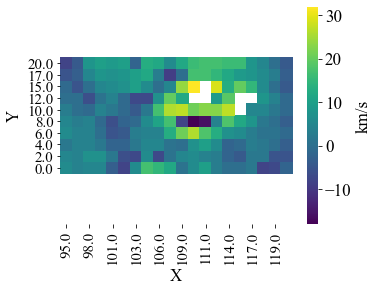
\includegraphics[width=2.5in]{Figures/6ISIS.png}
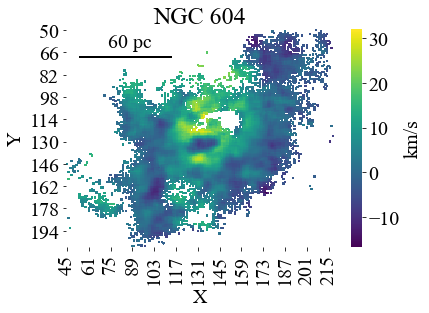
\includegraphics[width=2.5in]{Figures/M6T}
\caption{Radial velocity maps of NGC 604 in H$\alpha$. Above: ISIS observations. Below: TAURUS observations. }
\label{fig:M604}
\end{figure}

\begin{figure}
\centering 
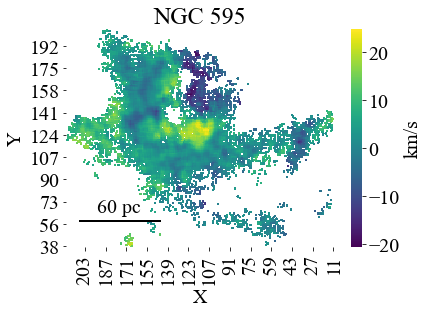
\includegraphics[width=2.5in]{Figures/M5T.png}
\caption{Radial velocity maps of NGC 595 in H$\alpha$.}
\label{fig:M595}
\end{figure}

\begin{figure}
\centering 
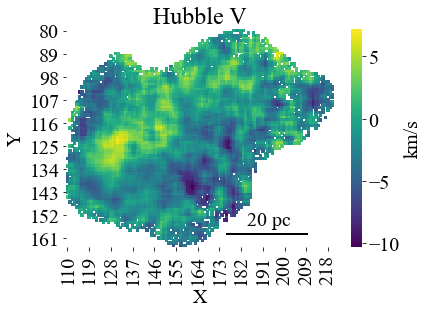
\includegraphics[width=2.5in]{Figures/MV.png}
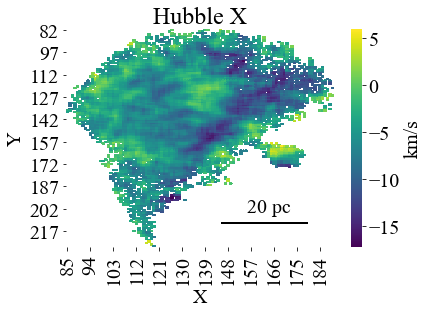
\includegraphics[width=2.5in]{Figures/MX.png}
\caption{Radial velocity maps of Hubble V and Hubble X in H$\alpha$.}
\label{fig:MHub}
\end{figure}



\section{Results}\label{sec:res}

Table \ref{tab:Res} shows the parameters we use to analyze our results. These are, the parameters obtained with a power-law fit of the structure function the index, m$_{2D}$, and the correlation length, l$_{0}$ and the ratio L$_{b}$/l$_{0}$, where L$_{b}$ is the horizontal size in pc of our sample box.  

Figure \ref{fig:SF604} shows the structure function (Equation \ref{eq:S}) of NGC 604 for the H$\alpha$ emission line for the ISIS and TAURUS instruments. The $m_{2D}$ is 1.7 with a correlation length of 11 pc. The $\sigma$ for the ISIS instrument is 8.4 km/s and for TAURUS instrument is 7.3 km/s. The fit to the power-law of the structure function is performed over the scales of 4 to 11 pc. The structure functions keep going up to scales of 70 pc, above these value the structure function falls steeply for the ISIS. As \cite{arthur2016turbulence} mentioned, the more pronounced steeping for small scales, below 4 pc in our case, is due to the spatial resolution of the observations. In comparison with TAURUS values, ISIS values are higher but are able to maintain the form of the structure function. 

Figure \ref{fig:SF595} shows the structure function of NGC 595 for the H$\alpha$ emission line. The $m_{2D}$ is 1.7 with a correlation length of 11 pc. The $\sigma$ is 6.6 km/s. The values of the structure function rise until 30 pc. 

Figure \ref{fig:SFV} shows the structure function of Hubble V for the H$\alpha$ emission line. The $m_{2D}$ is 1.8 with a correlation length of 4 pc and a $\sigma$ of 2.8 km/s. The structure function values keep going up and reach a maximum at $\sim$28 pc.

Figure \ref{fig:SFX} shows the structure function of Hubble V for the H$\alpha$ emission line. The $m_{2D}$ is 1.7 with a correlation length of 4 pc. The $\sigma$ of the region is 3.6 km/s. For this region, the structure functions keeps its tendency of going up to a scale o $\sim$ 18 pc.

\begin{table}
\begin{center}\caption{Main results.}
\begin{tabular}{cccccc}\hline
Region   &  m$_{2D}$  & l$_{0}$ [pc] & $\sigma$ [km/s] & L$_{b}$ [pc]  & L$_{b}$/l$_{0}$ \\\hline
NGC 604 &     1.7   &     11       &    7.3         & 170  &  15.4 	\\
NGC 595 &      1.7   &     11      &    6.6        & 200  & 18.1 \\
Hubble V &   1.8   &     3       &    2.8      & 68  &     22.6  	\\
Hubble X &     1.7   &     5       &    3.6      & 61  &  12.2 	\\
\end{tabular}\label{tab:Res}
\end{center}
\end{table} 

\begin{figure}
\centering 
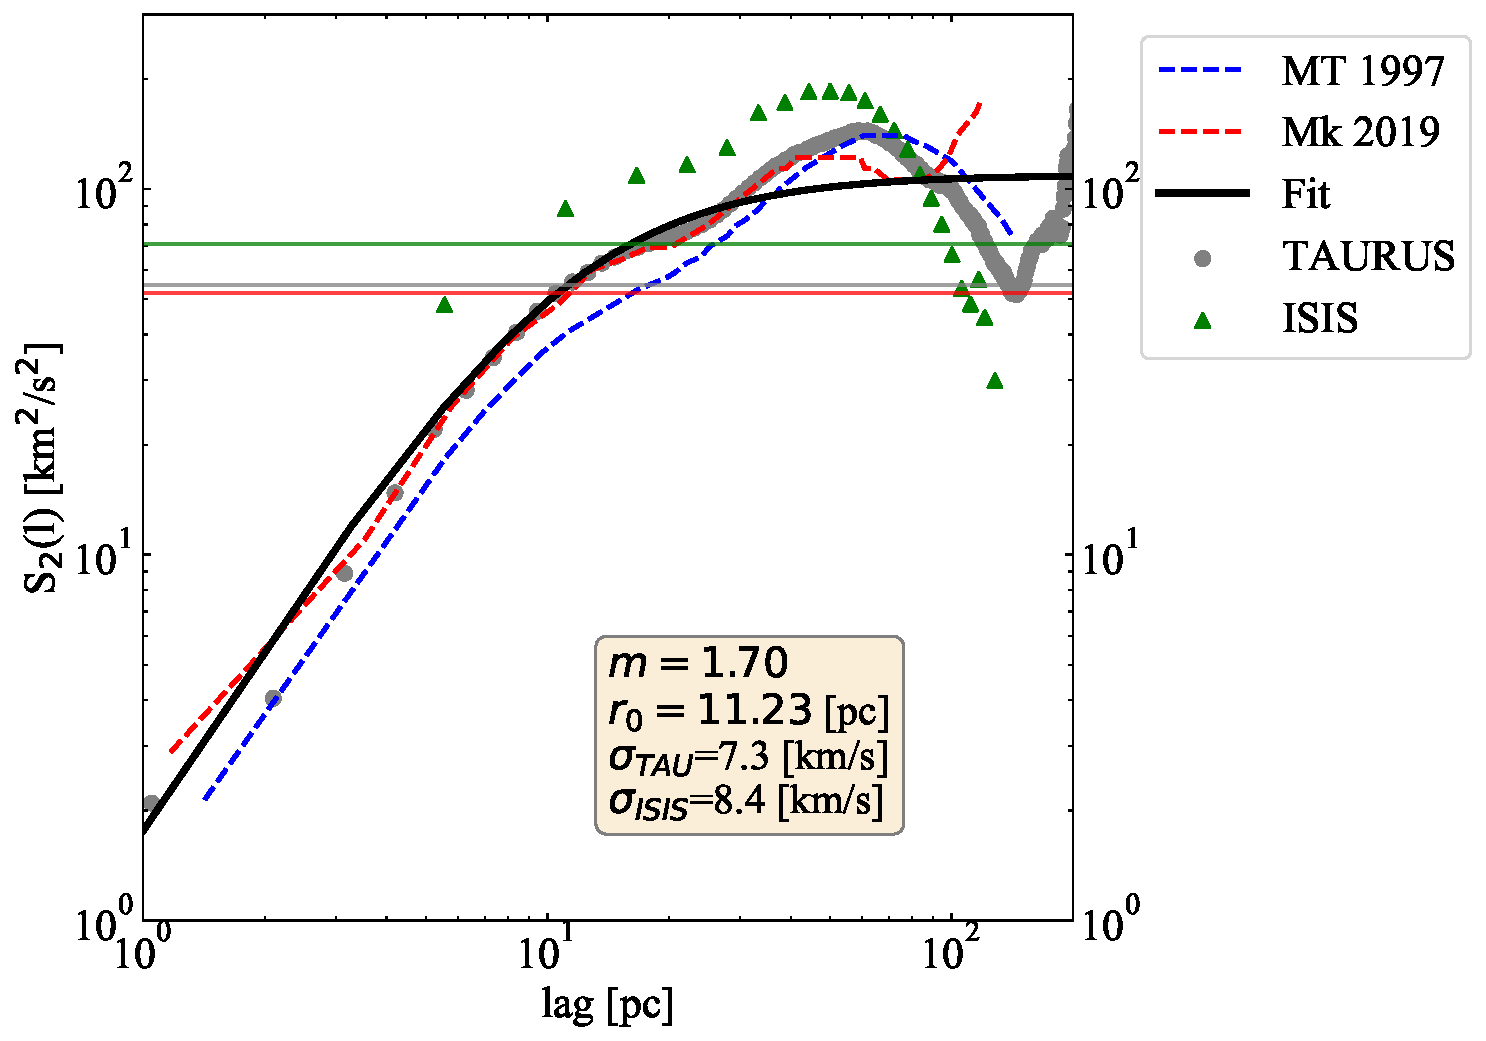
\includegraphics[width=3.5in]{Figures/SF604.pdf}
\caption{NGC 604 second-order structure functions for H$\alpha$ emission line for ISIS and TAURUS instruments. The figure also shows the structure functions presented in previous works. The green area represents the scales affected by observational seeing. The vertical line indicate the value of he correlation length. The horizontal line denote the value of $\sigma$.}
\label{fig:SF604}
\end{figure}

\begin{figure}
\centering 
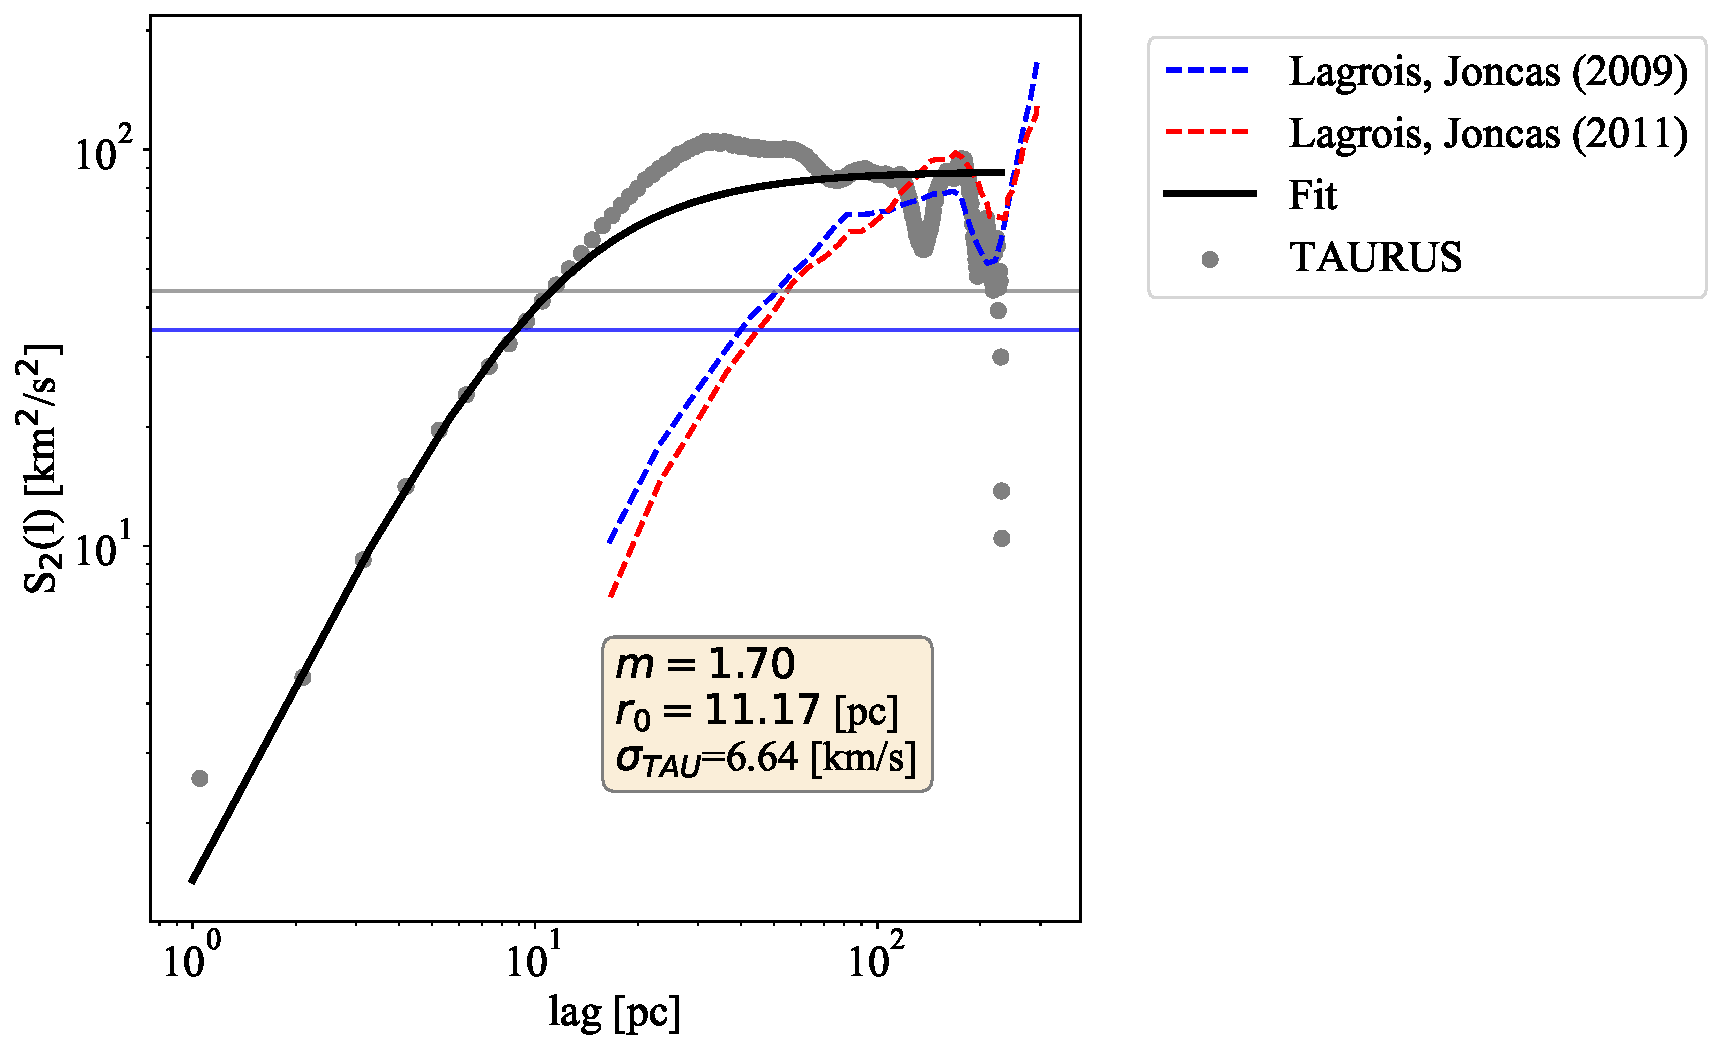
\includegraphics[width=4in]{Figures/SF595.pdf}
\caption{NGC 595 second-order structure functions for H$\alpha$ emission line for TAURUS instrument. The figure also shows the structure functions presented in previous works. Same information as Figure \ref{fig:SF604}.}
\label{fig:SF595}
\end{figure}

\begin{figure}
\centering 
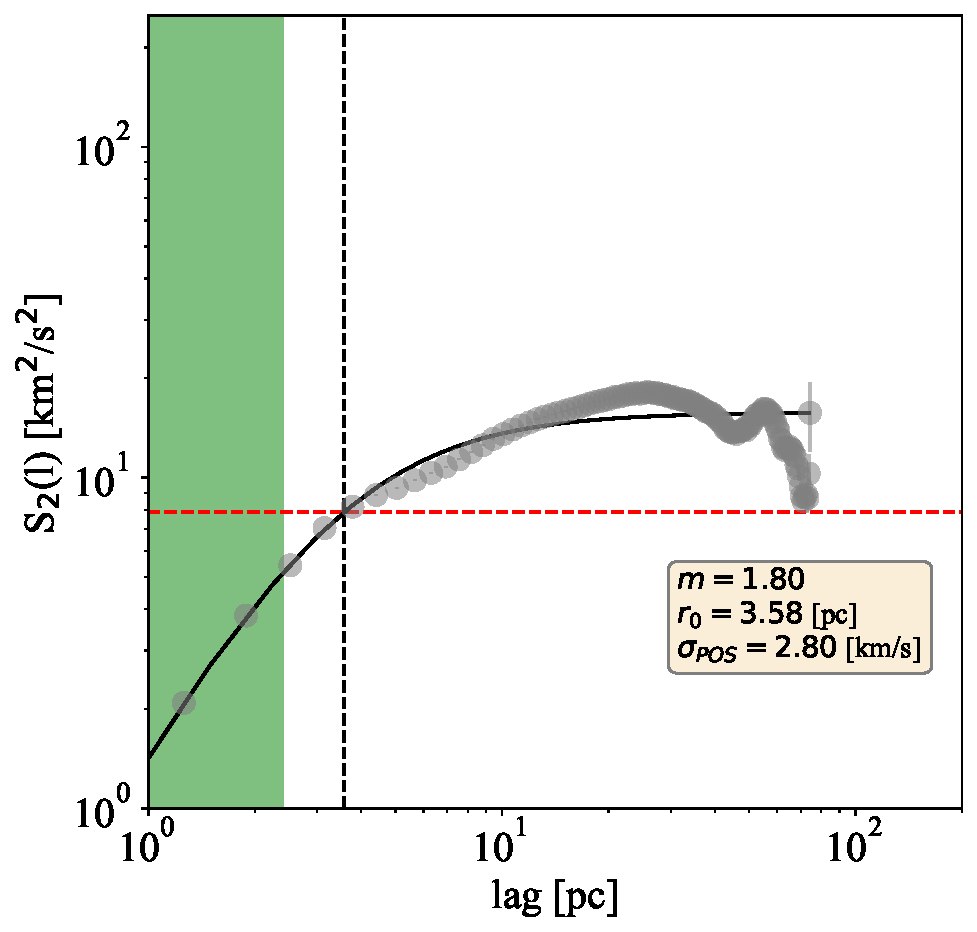
\includegraphics[width=2.5in]{Figures/SFHV}
\caption{Hubble V second-order structure functions for H$\alpha$ emission line for TAURUS instrument. Same information as Figure \ref{fig:SF604}.}
\label{fig:SFV}
\end{figure}

\begin{figure}
\centering 
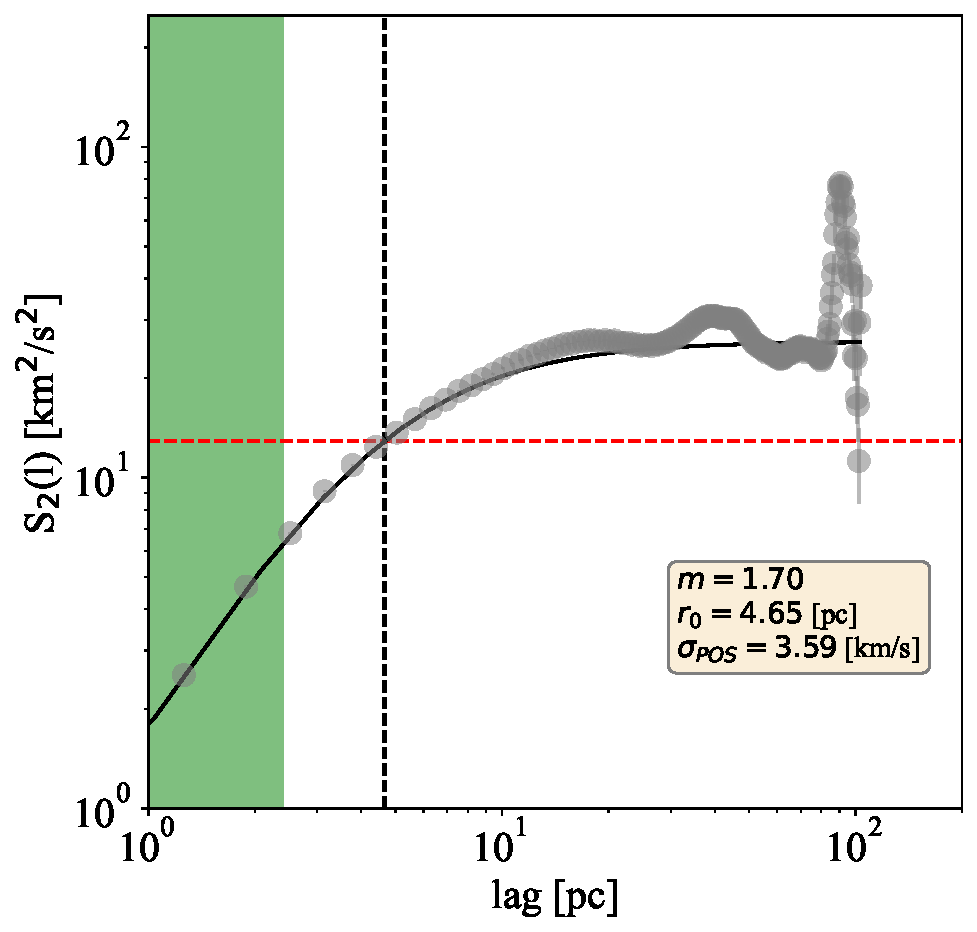
\includegraphics[width=2.5in]{Figures/SFHX}
\caption{Hubble X second-order structure functions for H$\alpha$ emission line for TAURUS instrument. Same information as Figure \ref{fig:SF604}.}
\label{fig:SFX}
\end{figure}

\clearpage

%%%%%%%%%%%%%%%%%%%%%%%%%%%%%%%%%%%%%%%%%%%%%%%%%%%%%%%%%%%%%%%%%%%%%%%%%%%%%%%%%%%%%%%%%%%%%%%%%%%%%%

\section{Discussion}\label{sec:disc}

\subsection{Comparison with previous structure functions determinations}

In an idealized case, at scales larger than r$_{0}$ the structure function flattens as it tends towards the asymptotic value of 2$\sigma$ \citep{arthur2016turbulence}. Figure \ref{fig:SF604} shows that the structure functions for NGC 604, except for \cite{2019arXiv191203543M}, follow a periodic behavior around 2$\sigma$. Using as reference the TAURUS results, the wave starts at 35 pc with a series of $ >$2$\sigma$ values up to $\sim$100 pc. Then $<$2$\sigma$ values follow until the largest scales of 150 pc. Therefore this periodic behavior is related to scales of $\sim$100 pc across our sample box. 

For NGC 595, above 30 pc a random pattern is around 2$\sigma$. Also, we can see this behavior for Hubble V, above 28 pc and Hubble X above 18 pc.

Figure \ref{fig:SF604} shows similarity in the TAURUS results and previous works \citep{tanco1997,2019arXiv191203543M}. The agreement lies that observations are the same but the procedure of calculating the structure function is different. \citep{2019arXiv191203543M} has $\sigma$ of 7.2 while we have 7.3 km/s. We note that our structure function results are more similar to \cite{2019arXiv191203543M} but the periodic behavior is strongly reduced on their results. \citep{tanco1997} also show this periodic pattern at large scales.

Figure \ref{fig:SF595} shows how there is no correspondence between our results and previous investigations. Our observations cover the brightest part of the region and have smaller resolution. \citet{lagrois2011} structure function results does not cover scales $<$10 pc.


%%%%%%%%%%%%%%%%%%%%%%%%%%%%%%%%%%%%%%%%%%%%%%%%%%%%%%%%%%%%%%%%%%%%%%%%%%%%%%%%%%%%%%%%%%%%%%%%%%%%%%

\section{Conclusions}\label{sec:concl}

\begin{enumerate}
    \item The giant HII regions in  M 33, NGC 604 and NGC 595 shows the same index and correlation lengths of 1.7 and 11 pc. These despite the noted differences on their physical properties and stellar populations. For NGC 604 wee find agreement in the structure function results between our data and previous publications. For NGC 595 our results are different from previous structure functions.
    
    \item Structure functions are presented for the first time for Hubble X and Hubble V, in NGC 6822. Hubble V shows and index of 1.8 and a correlation length of 4 pc, while Hubble X results are 1.7 and 5 pc.
    
\end{enumerate}

%%%%%%%%%%%%%%%%%%%%%%%%%%%%%%%%%%%%%%%%%%%%%%%%%%%%%%%%%%%%%%%%%%%%%%%%%%%%%%%%%%%%%%%%%%%%%%%%%%%%%%

\section*{Acknowledgements}

The Acknowledgements section is not numbered. Here you can thank helpful
colleagues, acknowledge funding agencies, telescopes and facilities used etc.
Try to keep it short.

%%%%%%%%%%%%%%%%%%%%%%%%%%%%%%%%%%%%%%%%%%%%%%%%%%
%%%%%%%%%%%%%%%%%%%% REFERENCES %%%%%%%%%%%%%%%%%%

\bibliographystyle{mnras}
\bibliography{bibphd}

%%%%%%%%%%%%%%%%%%%%%%%%%%%%%%%%%%%%%%%%%%%%%%%%%%
%%%%%%%%%%%%%%%%% APPENDICES %%%%%%%%%%%%%%%%%%%%%
%%%%%%%%%%%%%%%%%%%%%%%%%%%%%%%%%%%%%%%%%%%%%%%%%%

% Don't change these lines
\bsp	% typesetting comment
\label{lastpage}
\end{document}

% End of mnras_template.tex